%\documentclass[12pt,a4paper]{report}
%\usepackage[utf8]{inputenc}
%\usepackage{amsmath}
%\usepackage{amsfonts}
%\usepackage{amssymb}
%\usepackage[margin=2.5cm]{geometry}
%\usepackage{graphicx}
%\usepackage{caption}
%\usepackage{subcaption}
%\usepackage[nottoc,numbib]{tocbibind}
%\linespread{1.3}
%\begin{document}
\chapter{The Zener Tunnelling Barrier}
\label{Asymmetrical Barrier}
	The Zener tunnelling barrier or "Zener barrier" \cite{b52} is a three region system similar to the potential barrier in Chapter \ref{Rectangular Barrier} with the exception that the constants in regions $a$ and $c$ are not equal. Zener tunnelling is the process whereby an electron may be excited from the valence band into the conduction band by a strong electric field \cite{b42,b43}. The Zener tunnelling in graphene nano-devices is represented by an electron-hole interface in the potential structure \cite{b48, b54}, which can be seen at energies within a potential step. The three region systems which include a potential step can be interpreted as a double step, or as a Zener barrier which consists of a barrier on top of a step.
	\begin{figure}[h]
		 \begin{subfigure}[h]{0.5\textwidth}
			\centerline{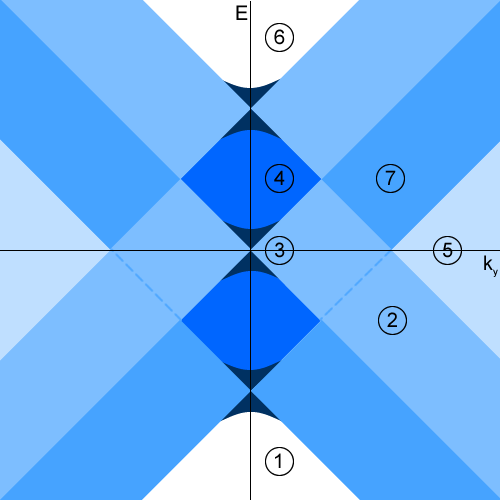
\includegraphics[scale=0.45]{images/asy-regions-flat}}
			\caption{}
		\end{subfigure}
		\hspace{0.5cm}
		\begin{subfigure}[h]{0.5\textwidth}
			\centerline{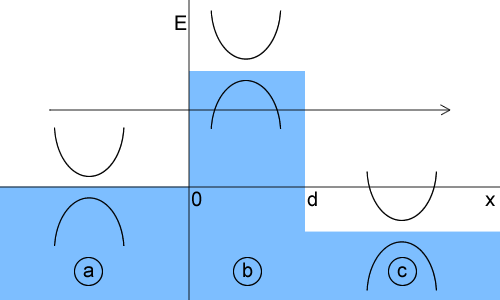
\includegraphics[scale=0.45]{images/asy-flat}}
			\caption{}
		\end{subfigure}
		\caption{(a) Transmission region diagram of energy against $k_{y}$ ($\hbar v_{f}=1$) for a three region Zener tunnelling system. Regions of transport (1, 4, 6), energy gap (3) and no propagation (2, 5, 7) are shown. (b) Diagram of a Zener tunnelling potential barrier in graphene, including energy spectrum in specific regions. Here a right travelling massive charge carrier is shown transmitting through a barrier with width $d$ and heights $V_{b}>V_{a}$ and $V_{c}<V_{a}$.}
		\label{asy-regions-flat}
	\end{figure}

	The transmission properties of the Zener barrier are shown in Figure \ref{asy-regions-flat} (a). In the same way as a symmetrical barrier regions 1, 4 and 6 are where electron-electron, electron-hole-electron or hole-hole transport occur, here it is expected that transmission is high as well as evidence of resonances and bound states. In region 3 the energy gap introduced into the graphene spectrum causes no transmission or no incident particles depending on the direction of the incident charge carrier. Region 5 can only be represented in Figure \ref{asy-regions-flat} (a). Here $\hbar v_{f} k_{y}>E$, therefore only imaginary solutions could exist. Regions 2 and 7 are regions where $\hbar v_{f} k_{y}>E$ but  $\hbar v_{f} k_{y}<E-V$, therefore there is no transmission here, but bound states can still be found for these regions.

%%%%%
%%%%%
%%%%%
%%%%%
%%%%%

	\section{Transfer Matrix}
	\label{Asymmetrical Barrier - Transfer Matrix}
		The scattering properties for the Zener barrier can be calculated in a similar way to the symmetrical barrier. Oscillatory wave-functions in all three regions allow a transfer matrix to be constructed, however as region $c$ differs from region $a$ the transmission probability will not simply be defined as $T=|t|^{2}$. Following on from the continuity of probability current calculation in Chapter \ref{Potential Step} the transmission probability will be calculated from $T=1-R$.

		To construct a transfer matrix the wave-functions in each region of Figure \ref{asy-regions-flat} (b) can be written in matrix form. Continuity of the wave-functions requires that at the first boundary located at $x=d_{1}$, the wave-function $\psi_{a}$ must be equal to $\psi_{b}$. Using the wave-functions from Section \ref{Wave-functions - Oscillitary} this can be written as:
		\begin{align}
			\left[\begin{array}{ccc}
				e^{iq_{a}d_{1}}&e^{-iq_{a}d_{1}}\\
				\alpha_{a}e^{iq_{a}d_{1}+i\theta_{a}}&-\alpha_{a}e^{-iq_{a}d_{1}-i\theta_{a}}
			\end{array}\right]
			\left[\begin{array}{ccc}
				a_{1}\\
				a_{2}
			\end{array}\right]
			&=
			\left[\begin{array}{ccc}
				e^{iq_{b}d_{1}}&e^{-iq_{b}d_{1}}\\
				\alpha_{b}e^{iq_{b}d_{1}+i\theta_{b}}&-\alpha_{b}e^{-iq_{b}d_{1}-i\theta_{b}}
			\end{array}\right]
			\left[\begin{array}{ccc}
				a_{3}\\
				a_{4}
			\end{array}\right]
		\end{align}
		Where the matrices $m_{1}$ and $m_{2}$ represent the wave-functions in matrix form to the left and right of the barrier interface so that:
		\begin{align}
			m_{1}\left[\begin{array}{ccc}
				a_{1}\\
				a_{2}
			\end{array}\right]
			&=
			m_{2}\left[\begin{array}{ccc}
				a_{3}\\
				a_{4}
			\end{array}\right]
		\end{align}
		The continuity of wave-functions requires that at the second boundary $x=d_{2}$, the wave-function $\psi_{b}$ must be equal to $\psi_{c}$:
		\begin{align}
			\left[\begin{array}{ccc}
				e^{iq_{b}d_{2}}&e^{-iq_{b}d_{2}}\\
				\alpha_{b}e^{iq_{b}d_{2}+i\theta_{b}}&-\alpha_{b}e^{-iq_{b}d_{2}-i\theta_{b}}
			\end{array}\right]
			\left[\begin{array}{ccc}
				a_{3}\\
				a_{4}
			\end{array}\right]
			&=
			\left[\begin{array}{ccc}
				e^{iq_{c}d_{2}}&e^{-iq_{c}d_{2}}\\
				\alpha_{c}e^{iq_{c}d_{2}+i\theta_{c}}&-\alpha_{c}e^{-iq_{c}d_{2}-i\theta_{c}}
			\end{array}\right]
			\left[\begin{array}{ccc}
				a_{5}\\
				a_{6}
			\end{array}\right]
		\end{align}
		These wave-functions will then be abbreviated to $m_{3}$ and $m_{4}$ so that:
		\begin{align}
			m_{3}\left[\begin{array}{ccc}
				a_{3}\\
				a_{4}
			\end{array}\right]
			&=
			m_{4}\left[\begin{array}{ccc}
				a_{5}\\
				a_{6}
			\end{array}\right]
		\end{align}
		With these relations the constants $a_{3}$ and $a_{4}$ can be eliminated. The transfer matrix $M$ becomes:
		\begin{align}
			\left[\begin{array}{ccc}
				a_{5}\\
				a_{6}
			\end{array}\right]=M
			\left[\begin{array}{ccc}
				a_{1}\\
				a_{2}
			\end{array}\right]\hspace{1cm}
			M=m_{4}^{-1}m_{3}m_{2}^{-1}m_{1}
		\end{align}
		Using the properties of transfer and scattering matrices, the reflection and transmission coefficients are stated as:
		\begin{align}
			r=\frac{M_{12}}{M_{22}}
			\hspace{1cm}
			t=\frac{1}{M_{22}}
		\end{align}
		Using the matrix M, the barrier interfaces can be set to $d_{1}=0$ and $d_{2}=d$. The reflection and transmission coefficients can then be evaluated to:
		\begin{align}
			r&=\frac{e^{-2iq_{c}d}\left(i\sin(q_{b}d)\left(\alpha_{b}^{2}-\alpha_{a}\alpha_{c}e^{-i\theta_{a}-i\theta_{c}}\right)+\alpha_{b}\alpha_{c}e^{-i\theta_{c}}\cos(q_{b}d-\theta_{b})-\alpha_{a}\alpha_{b}e^{-i\theta_{a}}\cos(q_{b}d+\theta_{b})\right)}{i\sin(q_{b}d)\left(\alpha_{a}\alpha_{c}e^{i\theta_{c}-i\theta_{a}}-\alpha_{b}^{2}\right)+\alpha_{b}\alpha_{c}e^{i\theta_{c}}\cos(q_{b}d-\theta_{b})+\alpha_{a}\alpha_{b}e^{-i\theta_{a}}\cos(q_{b}d+\theta_{b})}
			\\
			t&=\frac{\alpha_{b}\alpha_{c}e^{-iq_{c}d+i\theta_{a}}2\cos(\theta_{b})\cos(\theta_{c})}{\alpha_{b}e^{i\theta_{a}}\left(\alpha_{b}\cos(q_{b}d+\theta_{b})+\alpha_{c}e^{i\theta_{c}}\cos(q_{b}d-\theta_{b})-i\sin(q_{b}d)\left(\alpha_{b}+\alpha_{c}e^{i\theta_{c}}\right)\right)}
		\end{align}
		The reflection probability $R=|r|^{2}$ for a Zener barrier becomes:
		\begin{equation}
			R=\frac{r_{1}r_{2}}{r_{3}r_{4}}
		\end{equation}
		where the following definitions have been introduced as:
		\begin{align}
			r_{1}&=\alpha_{a}e^{i\theta_{a}}\cos(q_{b}d+\theta_{b})-\alpha_{b}\alpha_{c}e^{i\theta_{c}}\cos(q_{b}d-\theta_{b})-i\sin(q_{b}d)\left(\alpha_{a}\alpha_{c}e^{i\theta_{a}+i\theta_{c}}-\alpha_{b}^{2}\right)
			\\
			r_{2}&=\alpha_{a}\alpha_{b}e^{i\theta_{c}}\cos(q_{b}d+\theta_{b})-\alpha_{b}\alpha_{c}e^{i\theta_{a}}\cos(q_{b}d-\theta_{b})+i\sin(q_{b}d)\left(\alpha_{a}\alpha_{c}-\alpha_{b}^{2}e^{i\theta_{a}+i\theta_{c}}\right)
			\\
			r_{3}&=\alpha_{b}\alpha_{c}\cos(q_{b}d-\theta_{b})+\alpha_{a}\alpha_{b}e^{i\theta_{a}+i\theta_{c}}\cos(q_{b}d+\theta_{b})+i\left(\alpha_{a}\alpha_{c}e^{i\theta_{a}}+\alpha_{b}^{2}e^{i\theta_{c}}\right)\sin(q_{b}d)
			\\
			r_{4}&=\alpha_{a}\alpha_{b}\cos(q_{b}d+\theta_{b})+\alpha_{b}\alpha_{c}e^{i\theta_{a}+i\theta_{c}}\cos(q_{b}d-\theta_{b})-i\left(\alpha_{b}^{2}e^{i\theta_{a}}+\alpha_{a}\alpha_{c}e^{i\theta_{c}}\right)\sin(q_{b}d)
		\end{align}
		Then using the relation $T=1-R$ the transmission probability evaluates to:
		\begin{equation}
			T=\frac{4\alpha_{a}\alpha_{b}^{2}\alpha_{c}\cos(\theta_{a})\cos(\theta_{c})\cos^{2}(\theta_{b})e^{i\theta_{a}+i\theta_{c}}}{r_{3}r_{4}}
			\label{asy-t}
		\end{equation}

		Density plots of the transmission probability show unique properties for the barrier depending on the direction of the step within the system. By comparison to the symmetrical barrier there are extra regions of transmission introduced where the step is outside of the barrier. These are shown at $E=-0.05$ eV in the examples in Figure \ref{asy-5}. The transmission probability depends on strongly on the magnitude and order of potentials in each region as these potentials control the direction of any steps and whether the device acts as a Zener barrier, or a double potential step. Regions of $\sim$zero transmission probability are controlled by the grouped constants $\alpha_{a,b,c}$. From these constants the transmission probability must become zero when $E=V_{a,b,c}$ or $\sim$zero when an energy gap is included. Outside of these energy limits the transmission probability will become one if the $k_{y}$ dependence is removed $\left(\theta_{a}=0\right)$.
		\begin{figure}[h]
			 \begin{subfigure}[h]{0.5\textwidth}
				\centerline{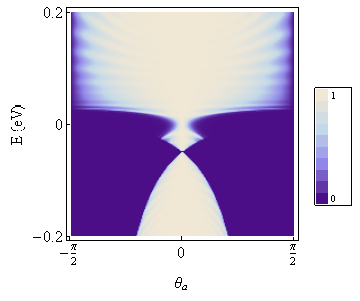
\includegraphics[scale=0.5]{images/asy-5}}
				\caption{The double step where $V_{a}=0.05$ eV, $V_{b}=0$ eV and $V_{c}=-V_{a}$.}
			\end{subfigure}
			\hspace{0.5cm}
			\begin{subfigure}[h]{0.5\textwidth}
				\centerline{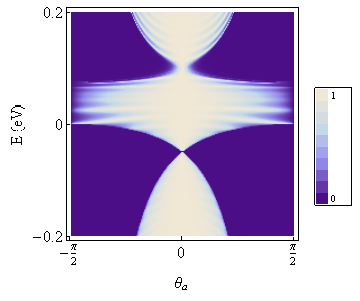
\includegraphics[scale=0.5]{images/asy-6}}
				\caption{The Zener barrier with $V_{a}=0.05$ eV, $V_{b}=0.1$ eV and $V_{c}=-0.05$ eV.}
			\end{subfigure}
			\caption{Density plot of transmission probability with energy against incident angle for the three region system in Equation (\ref{asy-t}). For both plots $d=200$ nm and  $m_{a,b,c}=0$ eV.}
			\label{asy-5}
		\end{figure}

		The introduction of an energy gap causes the transmission probability to become essentially zero at energies within the gap shown in Figure \ref{asy-1}. When no potential is included this produces a region of no transmission inside the gap and symmetrical transmission properties at energies outside of the gap. When both an energy gaps and potentials are included, the transmission probability becomes similar the potential barrier, however the regions of $\sim$zero transmission probability around $E=V_{a,b,c}$ increase to the size of the energy gap in that region. For small energy gaps a small transmission probability can be seen inside the gap.
		\begin{figure}[h]
			 \begin{subfigure}[h]{0.5\textwidth}
				\centerline{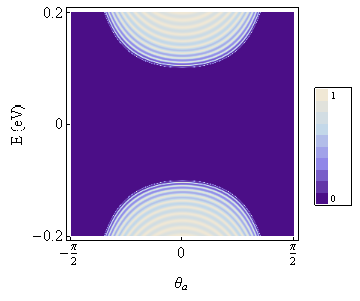
\includegraphics[scale=0.5]{images/asy-1}}
				\caption{Massive Zener barrier with $m_{a}=0.05$ eV, $m_{b}=0.1$ eV and $m_{c}=0$ eV.}
			\end{subfigure}
			\hspace{0.5cm}
			\begin{subfigure}[h]{0.5\textwidth}
				\centerline{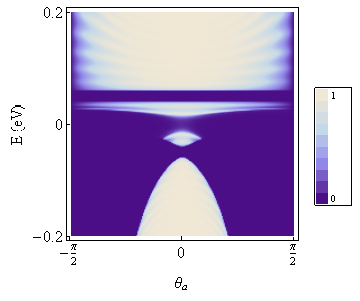
\includegraphics[scale=0.5]{images/asy-2}}
				\caption{The double step where $V_{a}=0.05$ eV, $V_{b}=0$ eV, $V_{c}=-V_{a}$ and $m_{a,b,c}=0.01$ eV.}
			\end{subfigure}
			\caption{Density plot of transmission probability with energy against incident angle for the three region system in Equation (\ref{asy-t}). For both plots $d=200$ nm.}
			\label{asy-1}
		\end{figure}
		\begin{figure}[h]
			 \begin{subfigure}[h]{0.5\textwidth}
				\centerline{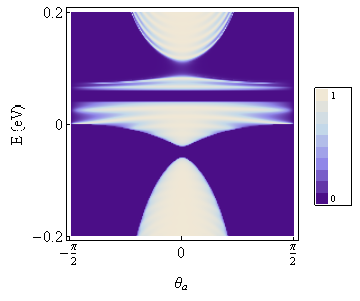
\includegraphics[scale=0.5]{images/asy-3}}
				\caption{The Zener barrier with $V_{a}=0.05$ eV, $V_{b}=0.1$ eV and $V_{c}=-0.05$ eV.}
			\end{subfigure}
			\hspace{0.5cm}
			\begin{subfigure}[h]{0.5\textwidth}
				\centerline{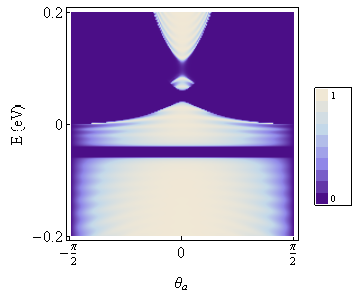
\includegraphics[scale=0.5]{images/asy-4}}
				\caption{The Zener barrier with $V_{a}=-0.05$ eV, $V_{b}=0.1$ eV and $V_{c}=0.05$ eV.}
			\end{subfigure}
			\caption{Density plot of transmission probability with energy against incident angle for the three region system in Equation (\ref{asy-t}). For both plots $d=200$ nm, $m_{a,b,c}=0.01$ eV.}
			\label{asy-3}
		\end{figure}
%%%%%
%%%%%
%%%%%
%%%%%
%%%%%
		\section{Resonances and Bound States}
		\label{Asymmetrical Barrier - Resonances and Bound States}
			The extra boundary at $x=d$ causes an additional reflected term into region $b$. This extra term allows the three region system to act as a Fabry-P\'{e}rot resonator. Under the resonance condition for a potential barrier $q_{b}d=n\pi$ \cite{b6} an expression for resonances inside the barrier can be obtained:
			\begin{equation}
				E=V_{b}\pm\sqrt{\hbar^{2}v_{f}^{2}\left(\frac{n^{2}\pi^{2}}{d^{2}}+k_{y}^{2}\right)+m_{b}^{2}}
				\label{resonances}
			\end{equation}
			When the resonance condition is applied to Equation (\ref{asy-t}) the expression for the transmission probability simplifies to:
			\begin{equation}
				T=\frac{4\alpha_{a}\alpha_{c}\cos(\theta_{a})\cos(\theta_{c})}{\alpha_{a}^{2}+\alpha_{c}^{2}+2\alpha_{a}\alpha_{c}\cos(\theta_{a}+\theta_{c})}
				\label{}
			\end{equation}
			This result is identical to Equation (\ref{stept}). This means that under resonance conditions the barrier becomes transparent, leaving only the step produced between regions $a$ and $c$ to scatter charge carriers. Similarly, the step like result occurs when examining the potential for Klein tunnelling. With large potentials $\theta_{b}=0$, $V_{b}\gg E$ and $\alpha_{b}=-1$. The transmission probability can then be reduced to:
			\begin{equation}
				T=\frac{4\alpha_{a}\alpha_{b}e^{i\theta_{a}+i\theta_{c}}\cos(\theta_{a})}{t_{1}t_{2}}
			\label{asy-klein}
			\end{equation}
			where the terms $t_{1}$ and $t_{2}$ are defined as:
			\begin{align}
				t_{1}&=-\cos(q_{b}d)\left(\alpha_{a}+\alpha_{c}e^{i\theta_{a}+\theta_{c}}\right)-i\sin(q_{b}d)\left(\alpha_{a}\alpha_{c}e^{i\theta_{c}}+e^{i\theta_{a}}\right)\\
						t_{2}&=i\sin(q_{b}d)\left(\alpha_{a}\alpha_{c}e^{i\theta_{a}}+e^{i\theta_{c}}\right)-\cos(q_{b}d)\left(\alpha_{c}+\alpha_{a}e^{i\theta_{a}+i\theta_{c}}\right)
			\end{align}
			The result for Klein tunnelling in Equation (\ref{asy-klein}) produces the plot in Figure \ref{asy-7}. This result shows step-like transmission properties with the addition of non-theta dependent resonances. The locations of these resonances can be found by applying the conditions for Klein tunnelling to the resonance condition. The resonance condition in Equation (\ref{resonances}) can then be modified with $V_{b}\gg\hbar v_{f}k_{y},m_{b}$ to find the resonances under Klein tunnelling:
			\begin{equation}
				E=V_{b}\pm \frac{\hbar v_{f}n \pi}{d}
			\end{equation}
			With the resonance condition the Klein tunnelling result in Equation (\ref{asy-klein}) further reduces to the transmission probability for the potential step.
			\begin{figure}[h]
				\centerline{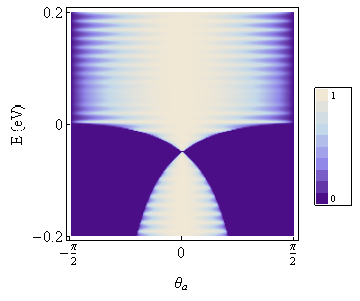
\includegraphics[scale=0.7]{images/asy-7}}
				\caption{Density plot of transmission probability and energy against incident angle from Equation (\ref{asy-klein}), showing the transmission probability through Zener barriers with large potentials. Here $V_{a}=0.05$ eV, $V_{b}\gg E$ and $V_{c}=-0.05$ eV.}
				\label{asy-7}
			\end{figure}

			The calculation in Section \ref{Rectangular Barrier - Bound States} to find bound states inside a potential barrier can be modified to apply to the Zener barrier. The energy spectrum for bound states in a Zener barrier is:
			\begin{equation}
				\tan(q_{b}d)=\frac{\alpha_{2}q_{b}\left(\alpha_{+}+\alpha_{-}\right)}{\alpha_{-}\alpha_{+}+\alpha_{2}k_{y}\left(\alpha_{+}-\alpha_{-}\right)-\alpha_{2}^{2}}
			\end{equation}
			
			However, as the wave-functions decay outside of the barrier region the asymmetry of this barrier structure has little effect on the bound states.
%%%%%
%%%%%
%%%%%
%%%%%
%%%%%
		\section{IV Characteristics at Finite Temperatures}
		\label{Asymmetrical Barrier - IV Characteristics at Finite Temperatures}
		Using the Landauer formalism from Section \ref{Introduction - Landauer Formalism in Graphene} the current through a graphene device can be obtained. The current depends on the gate voltage ($V_{g}$), source-drain voltage ($V_{sd}$) and temperature ($T$). The current can also be affected by the properties of the scattering region such as the step formed around the barrier ($V_{a,c}$) and any energy gap ($m$) in the spectrum of the charge carriers.

		It is clear from Figure \ref{asy-vg-3} that the current varies significantly depending on the step properties of the barrier. When $V_{a}>V_{c}$ the magnitude of the current can be seen to be over three times higher than the opposite step orientation. This result is in agreement with the current characteristics of the step potential; at $V_{g}=0$ eV the current coincides with the current from the step. At larger values for gate voltage the current shows less dependence, this is due to the barrier acting at energies much higher then the Fermi energy. When the source-drain voltage is reversed (as in  in Figure \ref{asy-vg-3} (c)) the current becomes negative and the direction of the step is reversed.
		\begin{figure}[h]
			 \begin{subfigure}[h]{0.3\textwidth}
				\centerline{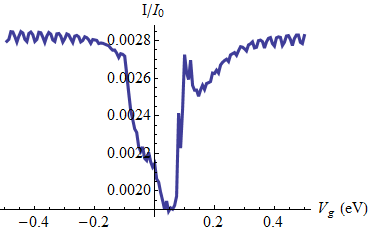
\includegraphics[scale=0.35]{images/asy-vg-3}}
				\caption{$eV_{sd}=0.1$ eV, $V_{a}=-0.1$ eV, $V_{b}=V_{g}$ and $V_{c}=0.1$ eV.}
			\end{subfigure}
			\hspace{0.5cm}
			\begin{subfigure}[h]{0.3\textwidth}
				\centerline{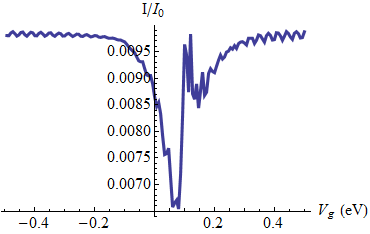
\includegraphics[scale=0.35]{images/asy-vg-4}}
				\caption{$eV_{sd}=0.1$ eV, $V_{a}=0.1$ eV, $V_{b}=V_{g}$ and $V_{c}=-0.1$ eV.}
			\end{subfigure}
			\hspace{0.5cm}
			\begin{subfigure}[h]{0.3\textwidth}
				\centerline{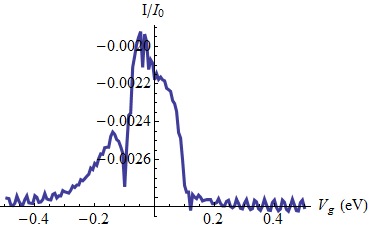
\includegraphics[scale=0.35]{images/asy-vg-5}}
				\caption{$eV_{sd}=-0.1$ eV, $V_{a}=0.1$ eV, $V_{b}=V_{g}$ and $V_{c}=-0.1$ eV.}
			\end{subfigure}
			\caption{Current against gate voltage from Equation (\ref{introduction-i-graphene}) with the transmission probability from Equation (\ref{asy-t}). The various graphene transistors were modelled with temperature $t=298$ K and width $d=100$ nm.}
			\label{asy-vg-3}
		\end{figure}

		When plotting the current against source-drain voltage properties from the step again become very apparent. Figure \ref{asy-v-1} shows the current as the source-drain is varied and as $V_{a}>V_{c}$ the current is much larger than for the opposite step direction for positive voltages. With negative source-drain voltages the current is less varied. As the step direction changes for negative voltages the IV curves could be expected to be mirrored, however, as the barrier is positive in both cases the current will not become fully symmetrical. 

		The lower current produced when $V_{a}<V_{c}$ does however result in an IV curve similar to that of a Zener diode. The negative voltage bias can be increased if an energy gap is included into the barrier region. This effect is shown in Figure \ref{asy-v-1} (c), which shows a strong negative bias.
		\begin{figure}[h]
			 \begin{subfigure}[h]{0.3\textwidth}
				\centerline{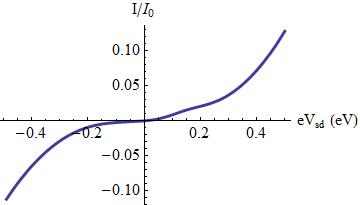
\includegraphics[scale=0.35]{images/asy-v-1}}
				\caption{$V_{a}=0.1$ eV, $V_{b}=0.2$ eV and $V_{c}=-0.1$ eV.}
			\end{subfigure}
			\hspace{0.5cm}
			\begin{subfigure}[h]{0.3\textwidth}
				\centerline{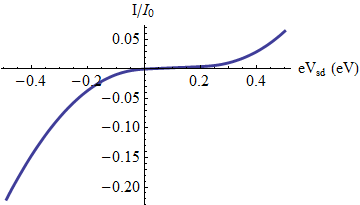
\includegraphics[scale=0.35]{images/asy-v-2}}
				\caption{$V_{a}=-0.1$ eV, $V_{b}=0.2$ eV and $V_{c}=0.1$ eV.}
			\end{subfigure}
			\hspace{0.5cm}
			\begin{subfigure}[h]{0.3\textwidth}
				\centerline{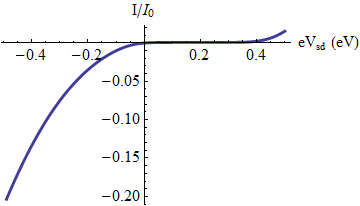
\includegraphics[scale=0.35]{images/asy-v-3}}
				\caption{$V_{a}=-0.1$ eV, $V_{b}=0.2$ eV, $V_{c}=0.1$ eV and $m_{b}=0.2$ eV.}
			\end{subfigure}
			\caption{Current against source-drain voltage from Equation (\ref{introduction-i-graphene}) with the transmission probability from Equation (\ref{asy-t}). The various graphene transistors were modelled with temperature $t=298$ K and width $d=100$ nm.}
			\label{asy-v-1}
		\end{figure}

		The currents dependence on temperature is shown in Figure \ref{asy-t-1}. While the $V_{a}<V_{c}$ case again shows a much higher overall current, it also shows current reduce as temperatures increase away from zero. As temperature increases; the temperature dependence becomes fairly linear as the energy contribution from temperature becomes greater than that of the voltages. Introducing an energy gap decreses the current at low temperatures. The example in Figure \ref{asy-t-1}(c) shows a large energy gap reducing the overall current and essentially removing the current at zero temperature.
		\begin{figure}[h]
			 \begin{subfigure}[h]{0.3\textwidth}
				\centerline{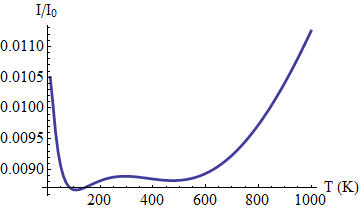
\includegraphics[scale=0.35]{images/asy-t-1}}
				\caption{$V_{a}=0.1$ eV, $V_{b}=0.2$ eV and $V_{c}=-0.1$ eV.}
			\end{subfigure}
			\hspace{0.5cm}
			\begin{subfigure}[h]{0.3\textwidth}
				\centerline{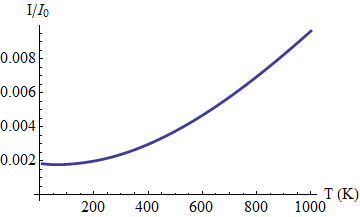
\includegraphics[scale=0.35]{images/asy-t-2}}
				\caption{$V_{a}=-0.1$ eV, $V_{b}=0.2$ eV and $V_{c}=0.1$ eV.}
			\end{subfigure}
			\hspace{0.5cm}
			\begin{subfigure}[h]{0.3\textwidth}
				\centerline{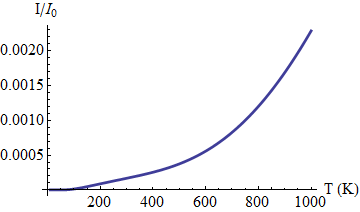
\includegraphics[scale=0.35]{images/asy-t-3}}
				\caption{$V_{a}=0.1$ eV, $V_{b}=0.2$ eV, $V_{c}=-0.1$ eV and $m_{b}=0.2$ eV.}
			\end{subfigure}
			\caption{Current against temperature from Equation (\ref{introduction-i-graphene}) with the transmission probability from Equation (\ref{asy-t}). The various graphene transistors were modelled with constant source-drain voltage $eV_{sd}=0.1$ eV and width $d=100$ nm.}
			\label{asy-t-1}
		\end{figure}
%%%%%
%%%%%
%%%%%
%%%%%
%%%%%
		\section{Conductance}
		\label{Asymmetrical Barrier - Conductance}
		The simplified zero-temperature, small voltage model in Equation (\ref{introduction-g-zero}) shows the dependence of conductance on the Fermi level. Again the two step directions shown in Figure \ref{asy-g-2} provide differing results; when $V_{a}>V_{c}$ energies within the barrier produce much larger conductances. Both cases produce linear dependence on Fermi energy outside of the potentials.
		\begin{figure}[h]
			 \begin{subfigure}[h]{0.3\textwidth}
				\centerline{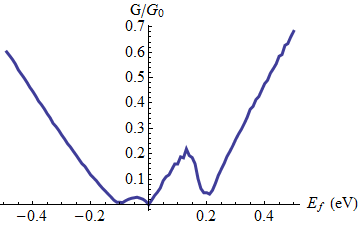
\includegraphics[scale=0.35]{images/asy-g-2}}
				\caption{$V_{a}=0.1$ eV, $V_{b}=0.2$ eV and $V_{c}=-0.1$ eV.}
			\end{subfigure}
			\hspace{0.5cm}
			\begin{subfigure}[h]{0.3\textwidth}
				\centerline{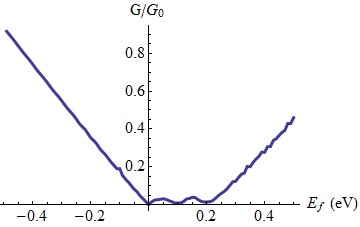
\includegraphics[scale=0.35]{images/asy-g-3}}
				\caption{$V_{a}=-0.1$ eV, $V_{b}=0.2$ eV and $V_{c}=0.1$ eV.}
			\end{subfigure}
			\hspace{0.5cm}
			\begin{subfigure}[h]{0.3\textwidth}
				\centerline{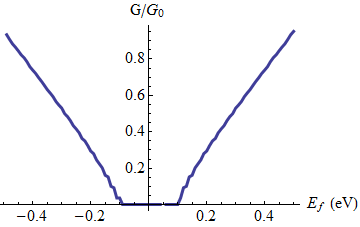
\includegraphics[scale=0.35]{images/asy-g-1}}
				\caption{$m_{a}=0.05$ eV, $m_{b}=0.1$ eV and $m_{c}=0$ eV.}
			\end{subfigure}
			\caption{The zero temperature conductance against Fermi-energy from Equation (\ref{introduction-g-zero}) with the transmission probability in Equation (\ref{asy-t}). The various graphene transistors were modelled with width $d=100$ nm and small source-drain voltages.}
			\label{asy-g-2}
		\end{figure}	
%\end{document}